\wde{
    Gaussian Distribution
}{
    We write $x \sim \mathcal{N}(\mu, \Sigma)$ to denote that $x$ is a random variable with mean $\mu$ and covariance $\Sigma$.
    It means that the probability density function of $x$ is given by
    $$
    p(x) = \frac{1}{2\pi^{d/2}|\Sigma|^{1/2}}\exp\left(-\frac{1}{2}(x-\mu)^T\Sigma^{-1}(x-\mu)\right)
    $$
}
\wde{Statistical Independence}{
    Two variables $x$ and $y$ are independent if 
    $$ 
    p(x,y) = p(x)p(y)
    $$
    Equivalently,
    $$
    p(x|y) = p(x)
    $$.
    The independence of $x$ and $y$ is denoted by $x \perp y$.
}
\wde{Statistical Independence [general]}
{
    If $\{x_1 , \ldots , x_n\} \perp \{y_1 , \ldots , y_m\}$ then
    $$
    p(x_1, \cdots, x_n, y_1, \cdots, y_m) = p(x_1, \cdots, x_n)p(y_1, \cdots, y_m)
    $$
}
\we{
    Factorisation of a joint distribution
}{
    Suppose $x \in \mathcal{X}, y \in \mathcal{Y}, z \in \mathcal{Z}$. If $\{x,y\} \perp z$ then
    $$
    p(x,y,z) = p(x,y)p(z)
    $$
    The original joint distribution (of size $|\mathcal{X}| \times |\mathcal{Y}| \times |\mathcal{Z}|$) can be factorised into two distributions of size $|\mathcal{X}| \times |\mathcal{Y}|$ and $|\mathcal{Z}|$.
}
\wde{Mutual Independence}{
    A set of variables $\{x_1, \ldots, x_n\}$ are mutually independent if
    $$
    p(x_1, \ldots, x_n) = \prod_{i=1}^n p(x_i)
    $$
}
\wde{Pairwise Independence}{
    A set of variables $\{x_1, \ldots, x_n\}$ are pairwise independent if
    $$
    p(x_i, x_j) = p(x_i)p(x_j)
    $$
    for all $i \neq j$.
}
\wt{Mutual Independence implies Pairwise Independence}{
    If a set of variables $\{x_1, \ldots, x_n\}$ are mutually independent, then they are pairwise independent.
    Converse is not true!
}
\wde{Conditional Independence}{
    The variables $x$ and $y$ are conditionally independent given $z$ if 
    $$
    p(x,y|z) = p(x|z)p(y|z)
    $$
    This is denoted by $x \perp y | z$.
}
\wde{Marginilisation}{
    The marginal distribution of $x$ is obtained by summing out all other variables.
    \begin{align*}
        p(x) &= \sum_y p(x,y) \\ 
        p(x | z) &= \sum_y p(x,y | z) \\
        p(x,y | z) &= p(x | z)p(y | z)
    \end{align*}
}
\wde{Bayes Rule}{
    Bayes rule is a way to invert conditional probabilities.
    $$
    p(x|y) = \frac{p(y|x)p(x)}{p(y)}
    $$
}
\wde{Chain Rule}{
    Any joint distribution can be factorised into a product of conditional distributions.
    $$
    p(x_1, \ldots, x_n) = p(x_1)p(x_2|x_1)p(x_3|x_1,x_2)\cdots p(x_n|x_1,\ldots,x_{n-1})
    $$
}
\wde{(directed) Graph Representation}{
    A directed graph is a set of nodes connected by edges.
    Each vertex is a random variable and each edge represents a direct dependency.
    It is directed and acyclic (DAG).
    A distribution factorises according to the graph if 
    $$
    p(x_1, \ldots, x_n) = \prod_{i=1}^n p(x_i | \text{parents}(x_i))
    $$
}
\wde{Graph structures}{
    \begin{itemize}
    \item Chain $x \perp z | y$
    \begin{center}
        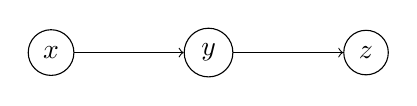
\begin{tikzpicture}
            \node[draw, circle] (x) at (0,0) {$x$};
            \node[draw, circle] (y) at (2,0) {$y$};
            \node[draw, circle] (z) at (4,0) {$z$};
            \draw[->] (x) -- (y);
            \draw[->] (y) -- (z);
        \end{tikzpicture}
    \end{center}
    \item Common cause $x \perp z | y$
    \begin{center}
        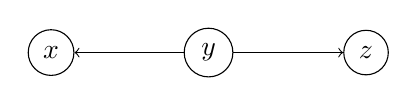
\begin{tikzpicture}
            \node[draw, circle] (x) at (0,0) {$x$};
            \node[draw, circle] (y) at (2,0) {$y$};
            \node[draw, circle] (z) at (4,0) {$z$};
            \draw[->] (y) -- (x);
            \draw[->] (y) -- (z);
        \end{tikzpicture}
    \end{center}
    \item v-structure $x \perp z$ but $x \not\perp z | y$
    \begin{center}
        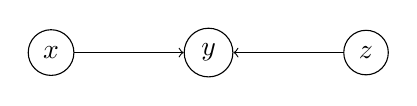
\begin{tikzpicture}
            \node[draw, circle] (x) at (0,0) {$x$};
            \node[draw, circle] (y) at (2,0) {$y$};
            \node[draw, circle] (z) at (4,0) {$z$};
            \draw[->] (x) -- (y);
            \draw[->] (z) -- (y);
        \end{tikzpicture}
    \end{center}
    \end{itemize}
}